% Chapter 4

\chapter{Trying to improve the State of the Art}

\lhead{Chapter 5. \emph{Trying to improve the State of the Art}} % This is for the header on each page - perhaps a shortened title
\label{chp:refwork}
%----------------------------------------------------------------------------------------

\def\:{\hskip0pt} %Definisce un modo veloce per permettere a latex di sillabare correttamente anche parole come 4-connectivity. Il corretto utilizzo è il seguente: 4\:-\:connectivity.
The architeture proposed by Cipriano et al. was quite simple yet effective. The
main novel addition was the use of a positional encoding. We now want to try to
improve the results obtained by them by adding some more complex
and more recent architectures, losses and optimizers.

\section{Boundary Loss}
Jointly with PosPadUNet3D, standard DICE loss was used. We also tried to use
CrossEntropy loss, but the results were not as good as with DICE loss so it has
been discarded. As we were dealing with higly unbalanced data, less than 1\% of
the whole volume is the canal, we looked for alternative losses which deal with
this problem.

Kervadec et al. proposed a loss function which takes the form of a distance
metric on the space of contours instead of regions. Dice or cross-entropy, are
based on regional integrals, which are convenient for training deep neural
networks. In practice, these regional integrals are summations over the
segmentation regions of differentiable functions, each directly invoking the
softmax probability outputs of the network. Therefore, standard stochastic
optimizers such as SGD are directly applicable. Unfortunately, difficulties
occur for highly unbalanced segmentations, for instance, when the size of target
foreground region is several orders of magnitude less than the background size,
which is a common charactiristic for medical images. The problem of such losses
is that thet assumes identical importance distribution for all the samples and
classes.

In the proposed paper, the authors proposed a new type of loss, named
\emph{Boundary loss} that aims to mitigate the issues related to regional losses
in highly unbalanced segmentation problems. Rather than using unbalanced
integrals over the regions, a boundary loss uses integrals over the boundary
between the regions. Furthermore, it provides information that is complementary
to regional losses. It is, however, challenging to represent the boundary points
corresponding to the regional softmax outputs of a CNN. This difficulty may
explain why boundary losses have been avoided in the context of deep
segmentation networks.

\subsection{Formulation}
The Boundary loss has been formulated as follows:
let $I: \Omega \subset \mathbb{R}^{2,3} \rightarrow \mathbb{R}$ denotes an image
with spatial domain $\Omega$, and $g: \Omega \rightarrow {0,1}$ a binary ground
thruth segmentation of the image such that $g(p) = 1$ if the pixel $p$ belongs
to the target region $G \subset \Omega$ and $0$ otherwise. Let $s_\theta :
\Omega \rightarrow [0,1]$ denotes the softmax probability output of a deep
segmentation network, and $S_\theta \subset \Omega$ denotes the corresponding
segmentation region: $\S_\theta = {p \in \Omega | s_\theta(p) >= \delta}$ for
some threshold $\delta$. Let $\Delta G$ denote a representation of the boundary
of ground-thruth region $G$ (i.e. the set of points of $G$, which have a spatial
neighbor in background $\Omega \setminus G$) and $\Delta S_\theta$ denoting the
boundary of the segmentation region defined by the network output.\\
The boundary loss can now be defined as:

\begin{equation}
  \label{eq:boundaryloss}
  \mathcal{L}_{\text{boundary}}(\theta) = \int_{\Omega} \phi_G(q)s_\theta(q)dq
\end{equation}

Where $\phi_G$ is the level set of the ground-thruth region $G$, obtained by
using the signed distance transform over $G$.

\subsection{Combining with other loss functions}
As we have already said, this type of loss is complementary to the regional
losses, since it provides information about the boundary of the segmentation
region, therefore they can be combined. In our experiments, we used the
following combination:
\begin{equation}
  \label{eq:boundaryloss}
  \mathcal{L}(\theta) = (1-\alpha)\mathcal{L}_{\text{boundary}}(\theta) + \alpha\mathcal{L}_{\text{DICE}}(\theta)
\end{equation}
Where $\alpha$ is a hyperparameter which weights the two losses.

Kervadec et al. in the paper where they presented this type of novel loss they
adopted a peculiar way to set this $\alpha$. As the training was kind of
unstable they set $\alpha$ to an inital value of $0$ and increased it's value by
$0.01$ and each training epoch until a fixed threshold. This type of approach
have given the best results in term of stability and performance thus we decided
to adopt it also in our experiments.

\section{PosDeepLab v3+}
DeepLab v3+ is another well known architecture for semantic segmentation. It
was proposed by Chen et al. in 2017 with the version 1 and is today still
improved. This architecture make use of the Atrous Spatial Pyramid Convolutions,
which are basically dilated convolutions in parallel and later concatenated,
each one with a different dilation rate.

\section{PosSegNet}
SegNet is a fully convolutional network for semantic segmentation. It was
proposed by Badrinarayanan et al. in 2015 and is structure in two parts: an
encoder and a decoder, similar to the one used in the U-Net. While the encoder
is made of convolutional layers followed by a max pooling. The indices of the
max pooling are stored in order to be used in the decoder during the upsampling.
Also in this case, the same positional encoding used in PosPadUNet3D was introduced.

\section{SwinUNETR3D}
Hatamizadeh et al. recently proposed a novel architecture for 3D medical image
segmentation which make use of the Transformer architecture. The main idea is to
replace the convolutions of U-Net used in the encoding phase with Transformer.
Instead of the standard Vision Transformer, Swin Transformer have been used as
they shown better performance on images. As Transformers are known to suffer
where there is lack of data, also a pre-training procedure has been proposed to
overcome this problem. In the following sections we will describe the proposed
architecture, starting from standard Transformer as proposed in the original
paper "Attention is all you need" by Vaswani et al. and then we will look at how
these ideas have been moved from NLP to Computer Vision.

\subsection{Transformer Architecture}
The transformer architecture were first introduced by Vaswani et al. in $2017$ in the field of Natural Language Processing.
The main idea is to replace a recurrent layers with a multi-head attention
mechanism, which is a linear operation that can be computed in parallel.
The attention mechanism is computed as follows:
\begin{equation}
  \label{eq:attention}
  \text{Attention}(Q,K,V) = \text{softmax}(\frac{QK^T}{\sqrt{d_k}})V
\end{equation}
Where $Q \in \mathbb{R}^{d_k}$ is the query, $K \in \mathbb{R}^{d_k}$ is the key
and $V \in \mathbb{R}^{d_v}$ is the value.
If we would like to make it multi-head, we add more attention layers in parallel
and concatenate the results. The final output of a multi-head attention layer is computed as follows:
\begin{equation}
  \label{eq:multiheadattention}
  \text{MultiHeadAttention}(Q,K,V) = \text{Concat}(\text{head}_1, \dots, \text{head}_h)W^O
\end{equation}
where $\text{head}_i = \text{Attention}(QW_i^Q, KW_i^K, VW_i^V)$.
The projection matrices $W_i^Q \in \mathbb{R}^{d_{\text{model}} \times d_k}$,
$W_i^K \in \mathbb{R}^{d_{\text{model}} \times d_k}$, $W_i^V \in
\mathbb{R}^{d_{\text{model}} \times d_v}$, and $W^O \in \mathbb{R}^{hd_v \times d_\text{model}}$ are learned parameters.
The complete architecture, which also add a residual connection, a linear layer
and a normalization layer, is shown in Figure \ref{fig:transformer}.
\begin{figure}[h]
  \centering
  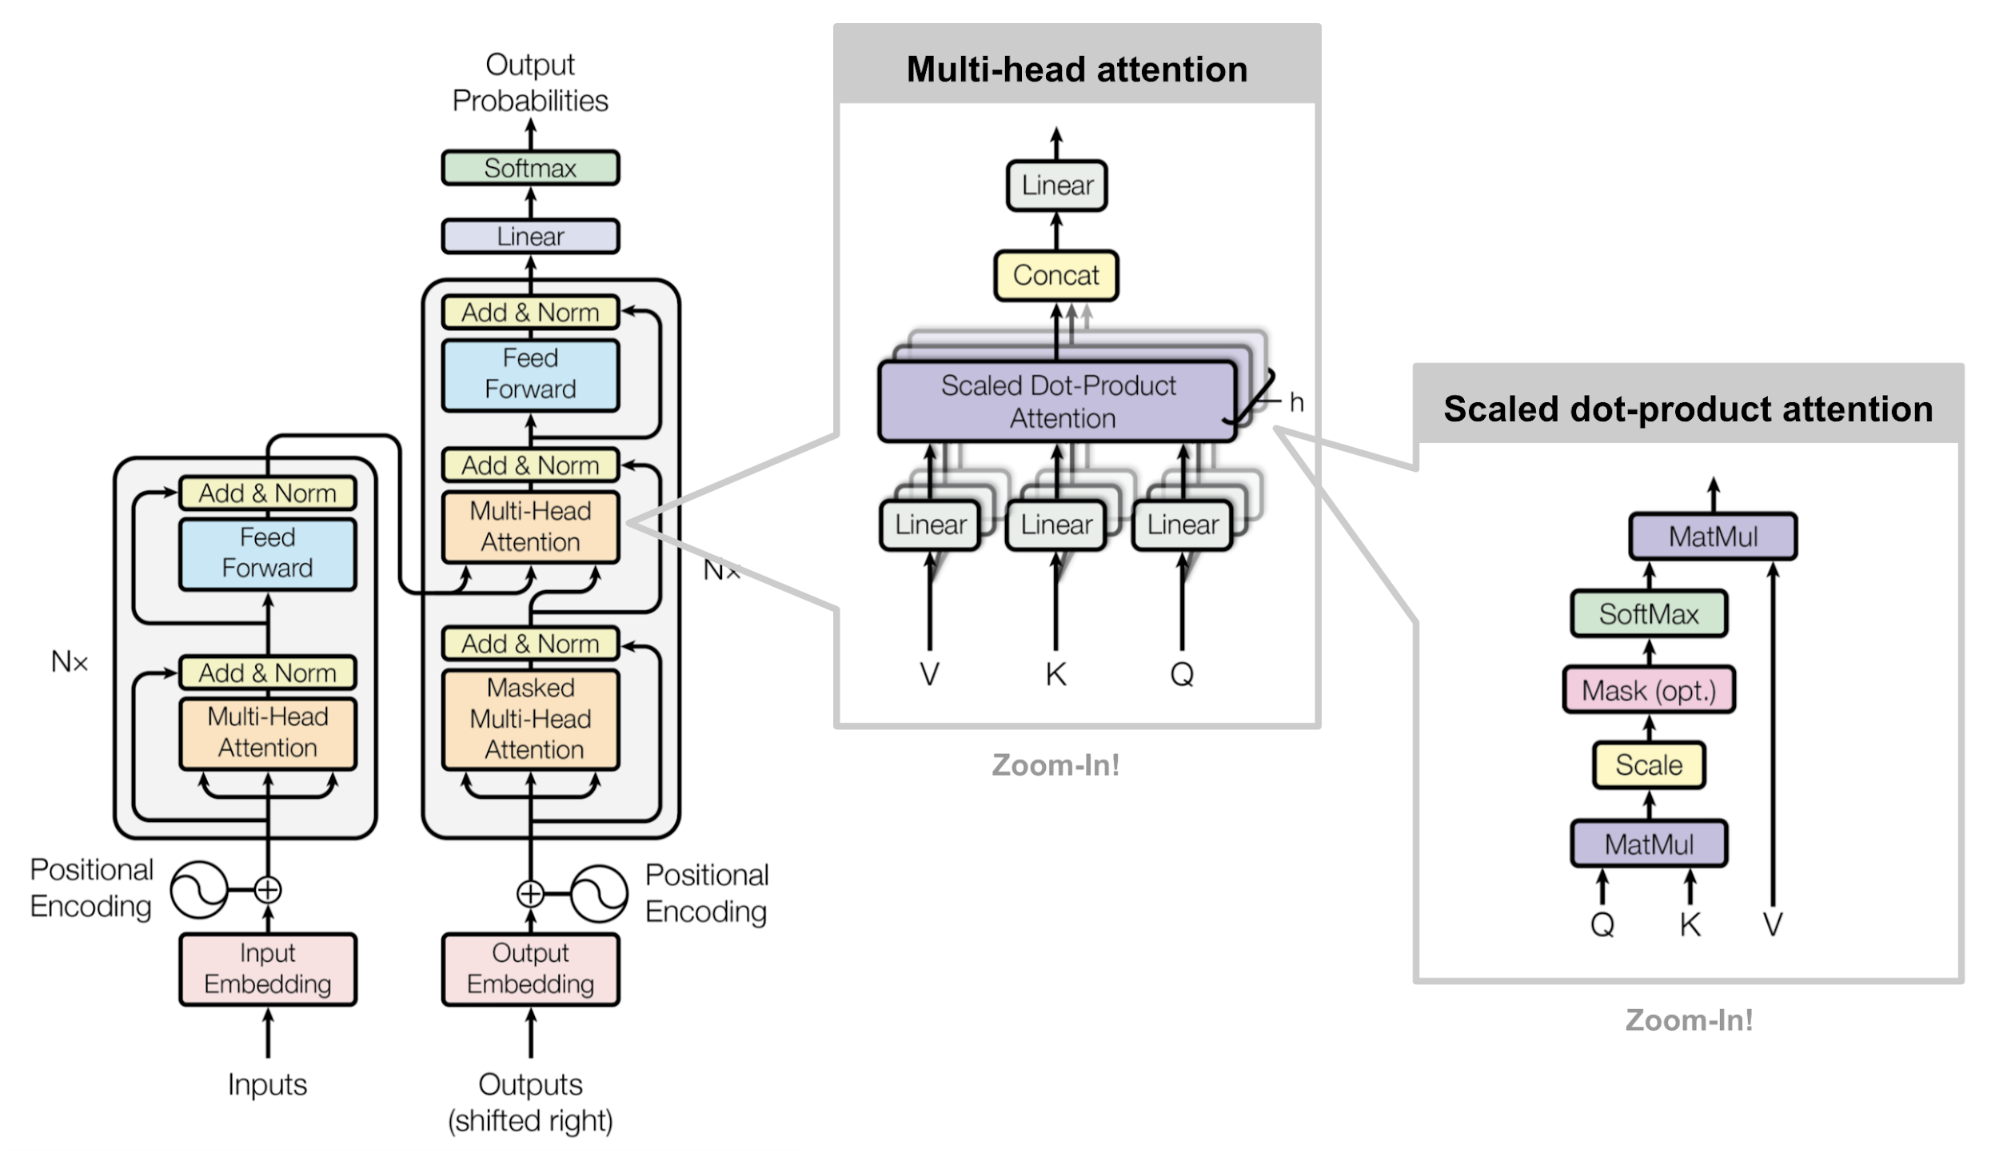
\includegraphics[width=0.8\textwidth]{transformer.png}
  \caption{Transformer architecture}
  \label{fig:transformer}
\end{figure}

\subsection{Vision Transformer}
While the Transformer architecture has become the de-facto standard for natural
language processing tasks, its applications to computer vision has remained
limited for few years. One of the reasons is that the complexity of the
attention mechanism is $O(n^2)$, where $n$ is the number of pixels in the image.
This makes it impractical for medium and large size images. In $2020$,
Dosovitskiy et al. proposed a novel architecture called Vision Transformer (ViT)
which is able to scale up the Transformer architecture to images. The main idea
is to reshape the original image $x \in \mathbb{R}^{H \times W \times C}$ into a
sequence of patches $x_p \in \mathbb{R}^{P \times P \times C}$, where $H$, $W$,
$C$ and $P$ are the height, width, number of channels and resolution of patches
respectively. The Transformer uses constant latent vector size $D$ through all
of its layers, so we flatten the patches and map to D dimensions with a
trainable linear projection. The outputs of such projections are the patch
embeddings. An additional token \texttt{[class]} is added to the sequence, which
is used to encode the class label of the image. The whole architecture is
depicted in Figure \ref{fig:visiontransformer}.

\begin{figure}[ht!]
  \centering
  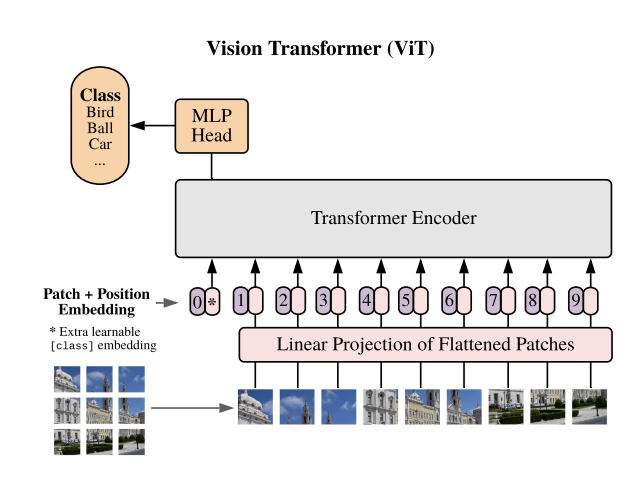
\includegraphics[width=0.5\textwidth]{Images/ViT.png}
  \caption{Vision Transformer architecture}
  \label{fig:visiontransformer}
\end{figure}


\subsection{Swin Transformer}
Swin Transformer, where the word \emph{Swin} stands for \emph{Shifted Window},
is a novel architecture proposed by Zhang et al. in $2021$ which has become
quite popular in the field of computer vision in this latter years. The problem
that the authors wanted to solve is that the Vision Transformer are not really
well suited for task which requires dense prediction at pixel level such as
semantic segmentation, so they propose a novel which constructs hierarchical
feature maps and has linear computational complexity to image size.

The Swin Transformer still relies on patches, but instead of choosing one size
and sticking with it, it first starts with small patches for the first
Transformer layer, then merges them into bigger ones in the deeper Transformer
layers. The first size chosen for the patches is $4 \times 4$ and then it is
projected to a chosen dimensionality $C$, which in the paper has been proposed
to be $96$ for the small model and $192$ for the large model. Then, these
vectors are processed with a Transformer which make used of a Shifted Window
based Self-Attention, introduced in this paper, intead of the classical
Self-Attention used in ViT. This type of attention has the benefit to be linear
because it is limited to a fixed number of patches $M$, so it's complexity will
be $O(M \times N)$ instead of $O(N^2)$ where $N$ is the number of patches.
The output of such Transformer Layer is fed in to a Merging Layer which
concatenates the vectors of groups of 2x2 neightboring patches and fed to
another Linear layer to reduce the dimensionality.
This process is repeated but for each layer, the region where the attention was
limited to is shifted in order to apply the attention to a different set of
patches, which before could not be seen among each other.

As a result, Swin Transformers are suitable for various downstream tasks wherein
the extracted multi-scale features can be leveraged for further processing.
\begin{figure}[ht!]
  \centering
  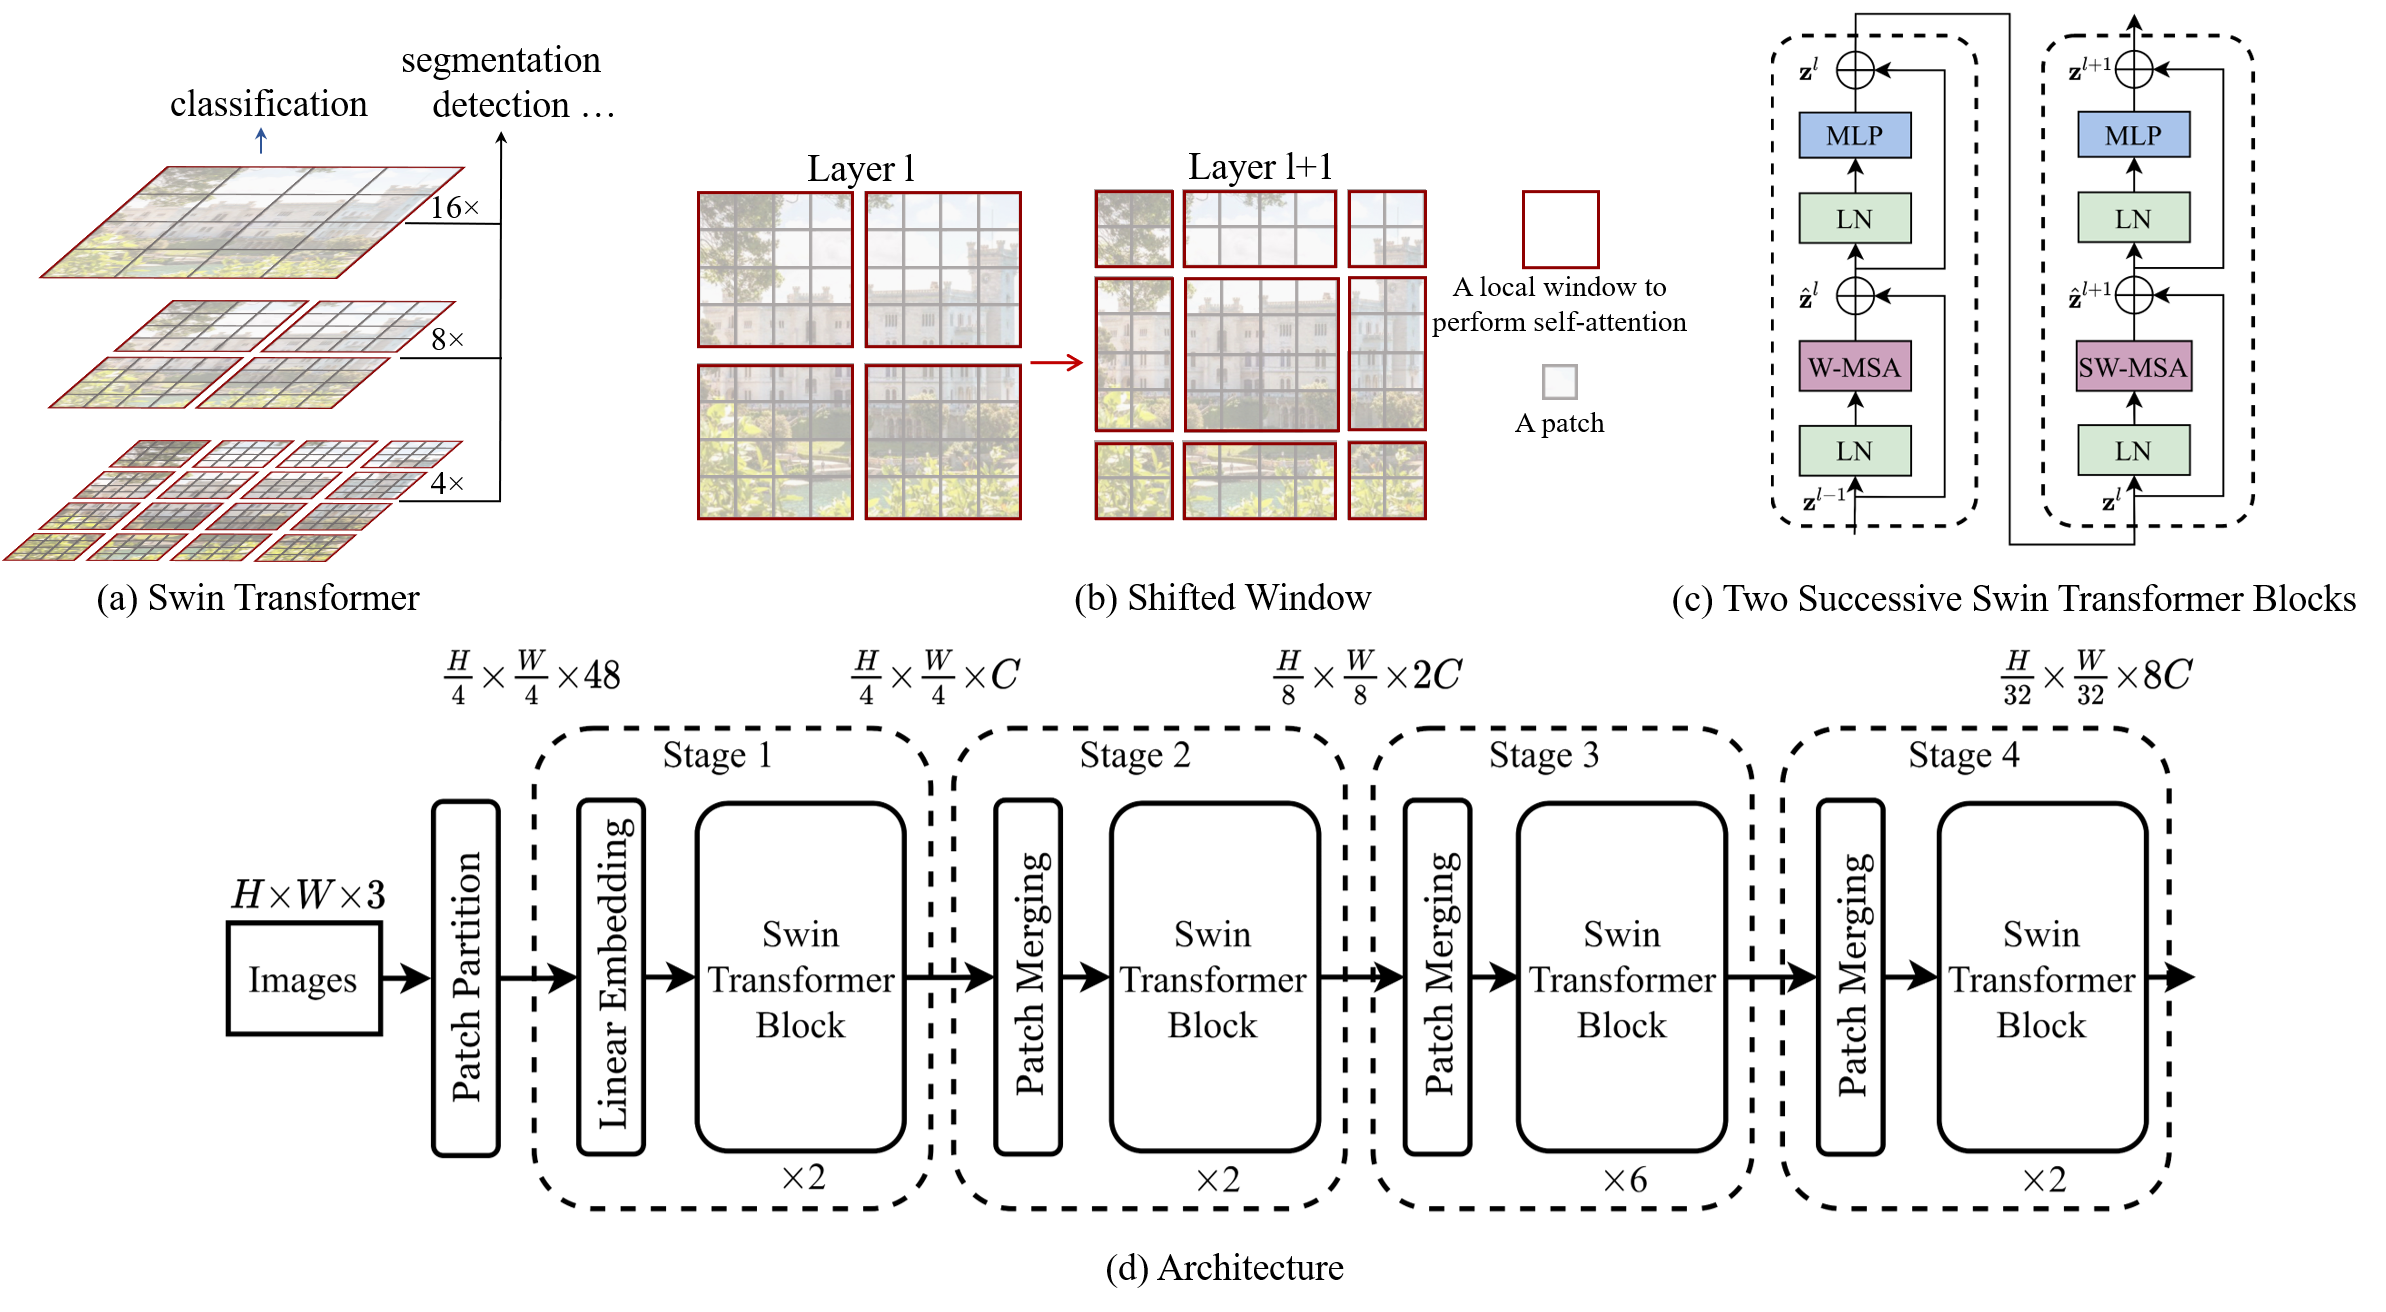
\includegraphics[width=0.8\textwidth]{Images/SwinTransformer.png}
  \caption{Swin Transformer components}
  \label{fig:swintransformer}
\end{figure}

\subsection{Final Architecture and pre-training}
The final architecture that have been proposed by Hatamizadeh et al. follows the
structure of U-Net3D, but in the encoder part, SwinTransformers are used instead
of the standard 3D Convolution. Some changes from the original paper has been
made in order to adapt the model to our type of data.
From the original volume of size $168 \times 280 \times 360$, we extract patches
of size $96 \times 96 \times 96$. These patches are fed in the SwinUNetr model
which is composed by a 4-stages Swin Transformer that act as the encoder part
and a sequence of transposed convolutions as decoder. For each stage of the
encoder part, a skip connection is added to the output of the decoder stage with
the same shape, like in the original U-Net architecture. The whole architecture
is shown in Figure \ref{fig:swinunetr}.

\begin{figure}[ht!]
  \centering
  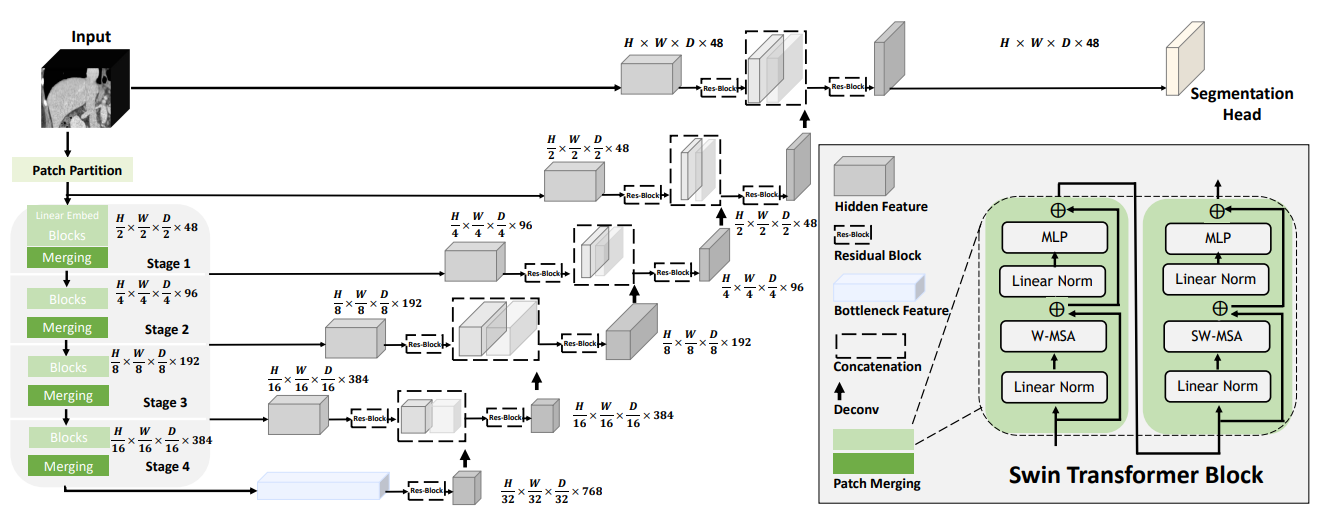
\includegraphics[width=0.8\textwidth]{Images/SwinUNETR.png}
  \caption{SwinUNETR architecture}
  \label{fig:swinunetr}
\end{figure}

As already mentioned, a pre-training phase is performed to overcome the data
hungriness charactiristic of Transformers. The pretraining has been performed by
paper authors on a variety of datasets of CT scans of different types have been
used. A total of 5 public CT datasets, consisting in a total of 5,050 subjects,
are used to construct the pre-training dataset. We do not tried to perform the
same pre-training on CBCT data instead of CT because the time required was
prohibitive.
The dataset used are:
\begin{itemize}
  \item{\textbf{Head \& Neck Squamous Cell Carcinoma (HNSCC)}: A collection
    contains imaging, radiation therapy, and clinical data from 627 head and
    neck squamous cell carcinoma (HNSCC) patients at MD Anderson Cancer Center.}
  \item{\textbf{Lung Nodule Analysis 2016 (LUNA 16)}: a collection of 888 CT
    scans of lung nodules.}
  \item{\textbf{TCIA CT Colonography Trial}: a collection of 825 CT colonography
    scans.}
  \item{\textbf{TCIA Covid 19}: a set of 2 dataset for a total 753 CT scans of
    the chest and annotation about the Covid-19 infection.}
  \item{\textbf{TCIA LIDC-IDRI}: a collection obtained by the collaboration of
    seven academic centers and eight medical imaging companies. It contains 1018
    cases of diagnostic and lung cancer screening thoracic computed tomography
    (CT) scans with marked-up annotated lesions.}
\end{itemize}

